\chapter{Procesos}

    A continuación, se muestran los procesos que se identifican para el presente proyecto, de los cuales se describe su objetivo, se da una descripción de dicho proceso y se proporciona el diagrama correspondiente.

    \section{Proceso de asignación}

        \subsection{Objetivo}

            Realizar la asignación de un NINI con alguna vacante de acuerdo al algoritmo diseñado.

        \subsection{Descripción}

            El proceso comienza cuando existe un nuevo registro ya sea de un becario o de alguna vacante, posteriormente el sistema realiza una consulta a las bases de datos para buscar los perfiles tanto del becario como los de las vacantes y proceder a realizar las asignaciones por medio del algoritmo de emparejamiento, si no se encuentra una `pareja' se le notifica que debe esperar y se le notificará cuando se encuentre una correspondencia.\\

            Si el sistema encuentra una "pareja" se procede a notificar tanto al NINI como a la empresa y se les proporcionan los datos respectivos para que se pongan en contacto, una vez que lleguen a un acuerdo ambos proceden a ingresar en el sistema  la aceptación de la asociación, entonces el sistema se encarga de retirar la vacante o disminuir el número de puestos disponibles en esa vacante, modificar el estado del becario y actualizar su historial, si alguno de los dos decide rechazar la asignación se le notificará al actor opuesto.

        \pagebreak
        \subsection{Diagrama}

            El diagrama correspondiente al proceso de Asignación se puede observar en la figura \ref{ProcesoAsignacion}.

            \begin{figure}[H]
                \begin{center}
                    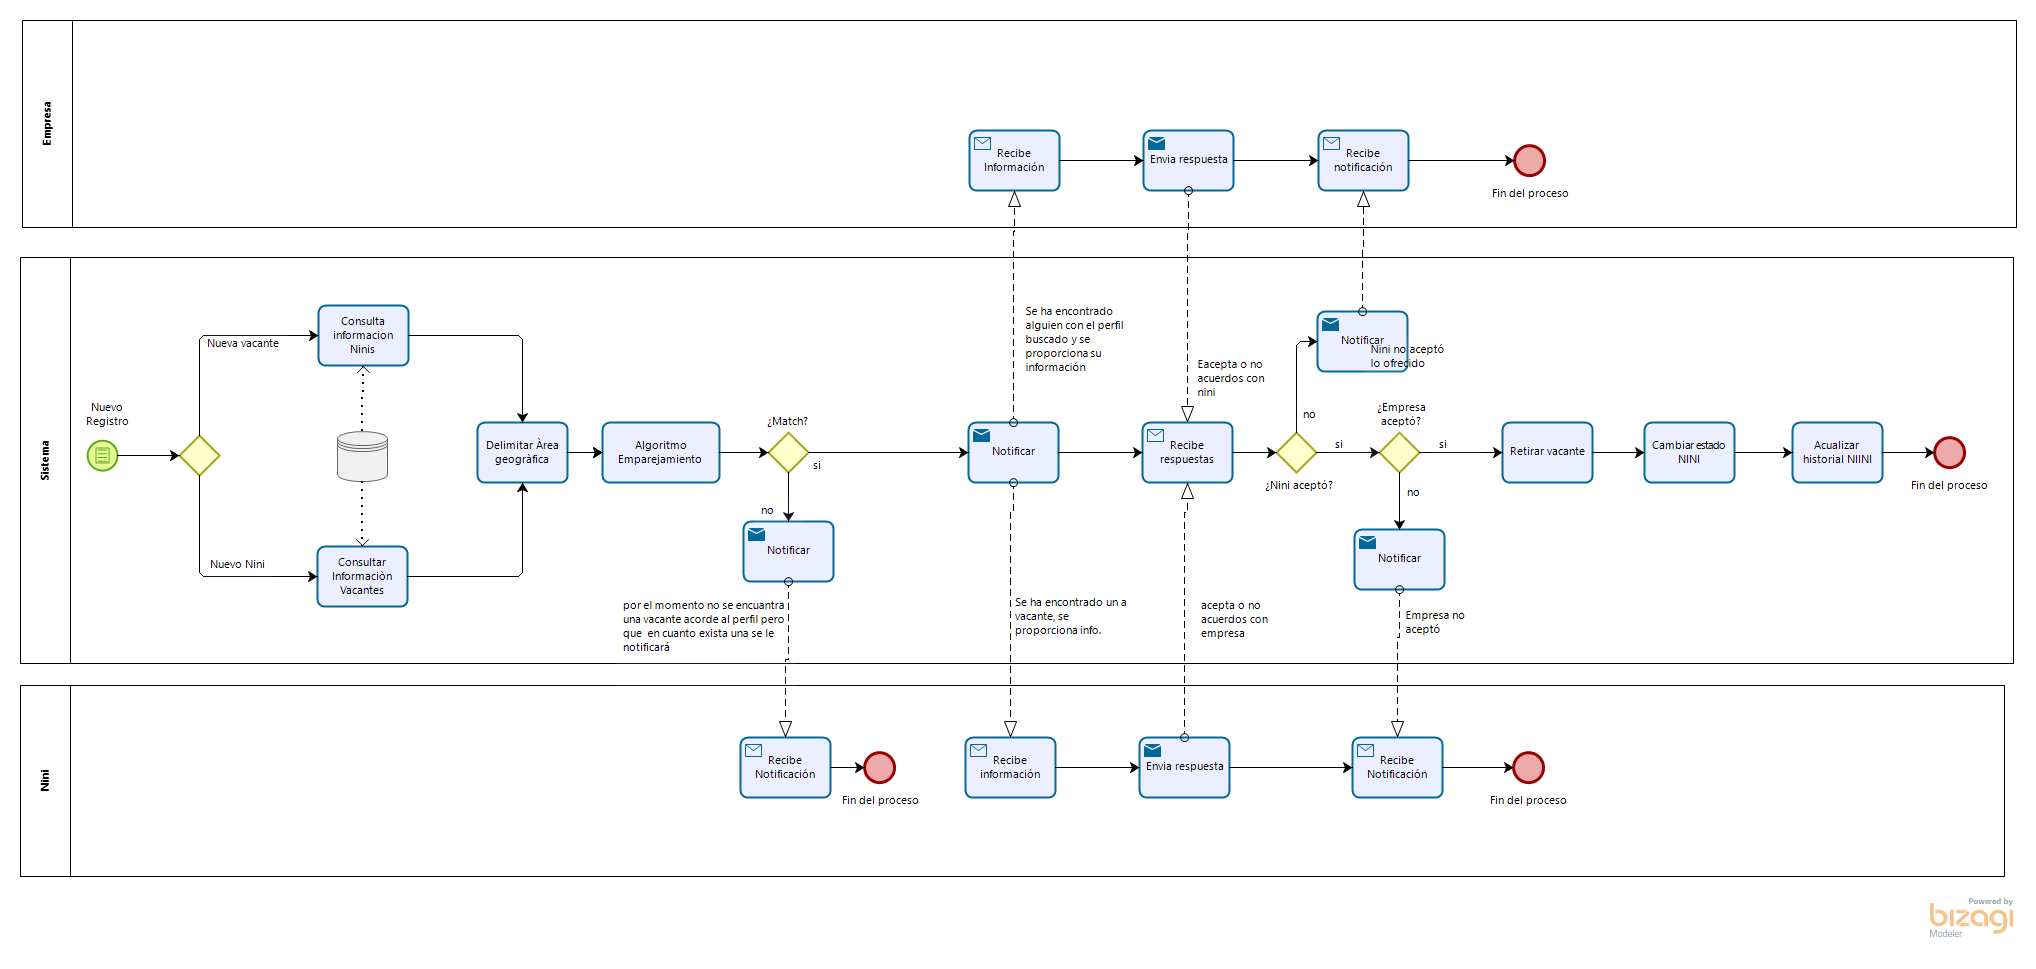
\includegraphics[angle=90, width=0.45\textwidth]{marcoTeorico/imagenes/Proceso-Asignacion.png}
                    \caption{Proceso ``Asignación''}
                    \label{ProcesoAsignacion}
                \end{center}
            \end{figure}



%\textbf{Tabla de Elementos del proceso}

%\begin{table}[htb]
%\centering
%\begin{tabular}{|l|l|}
%\hline
%\multicolumn{2}{|c|}{\textbf{Proceso Asignación}} \\ \hline
%\textbf{Procesos que dependen del proceso} &  Seguimiento \\ \hline


%\multirow{2}{*}{\textbf{Dependencia de otros procesos}} & Registro Ninis \\ %\cline{2-2}
%& Registro empresas \\ \hline

%\multirow{2}{3cm}{\textbf{Entradas}} & Datos nini \\ \cline{2-2}
%& Datos de vacantes \\ \hline

%\multirow{2}{3cm}{\textbf{Salidas}} & Notificaciones \\ \cline{2-2}
%& cambios de estado \\ \hline

%\multirow{2}{3cm}{\textbf{Precondiciones}} & Ninis Registrados \\ \cline{2-2}
%& vacantes registradas \\ \hline

%\multirow{2}{3cm}{\textbf{Postcondiciones}} & Retirar vacantes \\ \cline{2-2}
%& cambios de estado \\ \hline

%\end{tabular}
%\caption{Tabla de elementos.}
%\label{tabla:sencilla2}
%\end{table}





%%%%%%%%%%%%%%%%%%%%%%%%%%%%%%%%%%%%Registro Empresas
\newpage
\subsection{Proceso de registro de empresa}

\textbf{Objetivo} 

Realizar el registro de una empresa en el sistema.\\

\textbf{Diagrama} 
\begin{figure}[H]
\begin{center}
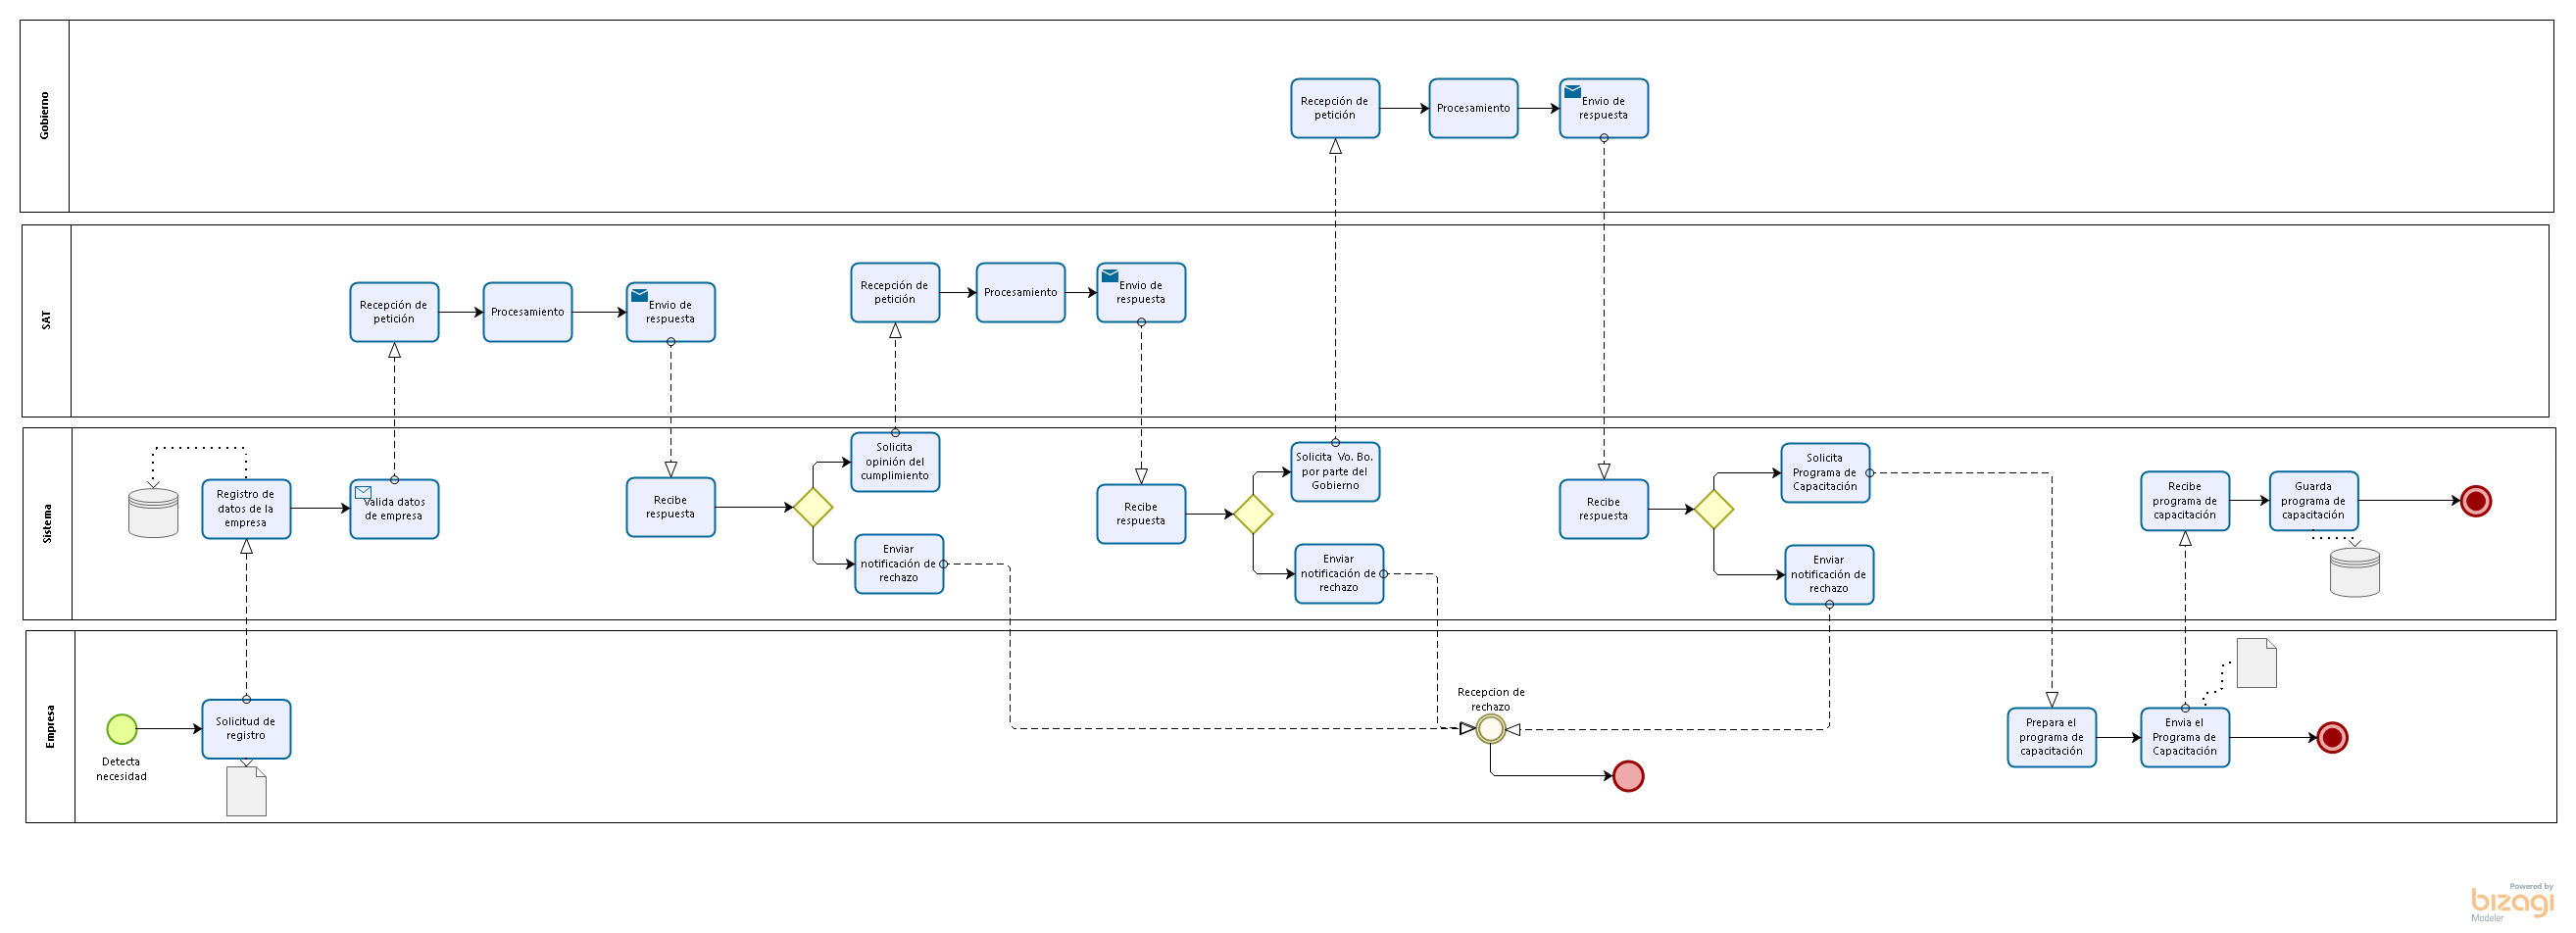
\includegraphics[angle=90, width=0.325\textwidth]{marcoTeorico/imagenes/Proceso_RegistroEmpresas.png}
\caption{Proceso ``Registro de empresa''}
\end{center}
\end{figure} 

\textbf{Descripción} \\

El proceso empieza cuando una empresa detecta una necesidad y requiere contratar personal, la empresa procede a realizar una solicitud de registro al sistema para lo cual ingresará su información y anexa los documentos que acreditan su registro como empresa (Cédula de identificación fiscal) y los documentos que permitan validar la identidad del representante de la empresa si es una persona moral o los documentos que avalen su propia identidad en caso de ser una persona física, una vez realizado esto se procede a realizar peticiones a servicios web (que serán simulados) para validar la información de la empresa con el SAT (Servicio de Administración Tributaria) para verificar el registro y conocer la “Opinión del cumplimiento”. Si la empresa cumple con la normatividad del SAT se procede a pedir el visto bueno del gobierno con la simulación del servicio web de la STPS (Secretaría del Trabajo y Previsión Social) para verificar la identidad del representante con la finalidad de continuar con el proceso.\\ \\
Después del visto bueno por parte del gobierno se solicita a la empresa su programa de capacitación para que se valide y guarde en la base de datos. \\

%\textbf{Tabla de Elementos del proceso}
%\begin{table}[htb]
%\centering
%\begin{tabular}{|l|l|}
%\hline
%\multicolumn{2}{|c|}{\textbf{Proceso Registro de Empresa}} \\ \hline
%\textbf{Procesos que dependen del proceso} &  Asignación \\ \hline

%\textbf{Dependencia de otros procesos} &  \\  \hline

%\multirow{2}{3cm}{\textbf{Entradas}} & Datos de la empresa \\ \cline{2-2}
%& Documentos para validar información \\ \hline

%\textbf{Salidas} & Notificaciones \\ \hline

%\textbf{Precondiciones} &  \\ \hline

%\textbf{Postcondiciones} & Empresa registrada \\ \hline

%\end{tabular}
%\caption{Tabla de elementos.}
%\label{tabla:sencillaEmpresas}
%\end{table}




%%%%%---------------------REGISTRO PERSONA

\newpage
\subsection{Proceso registro de becario}

\textbf{Objetivo} 

Realizar el registro de un becario en el sistema.\\
\newpage
\textbf{Diagrama} 
\begin{figure}[H]
\begin{center}
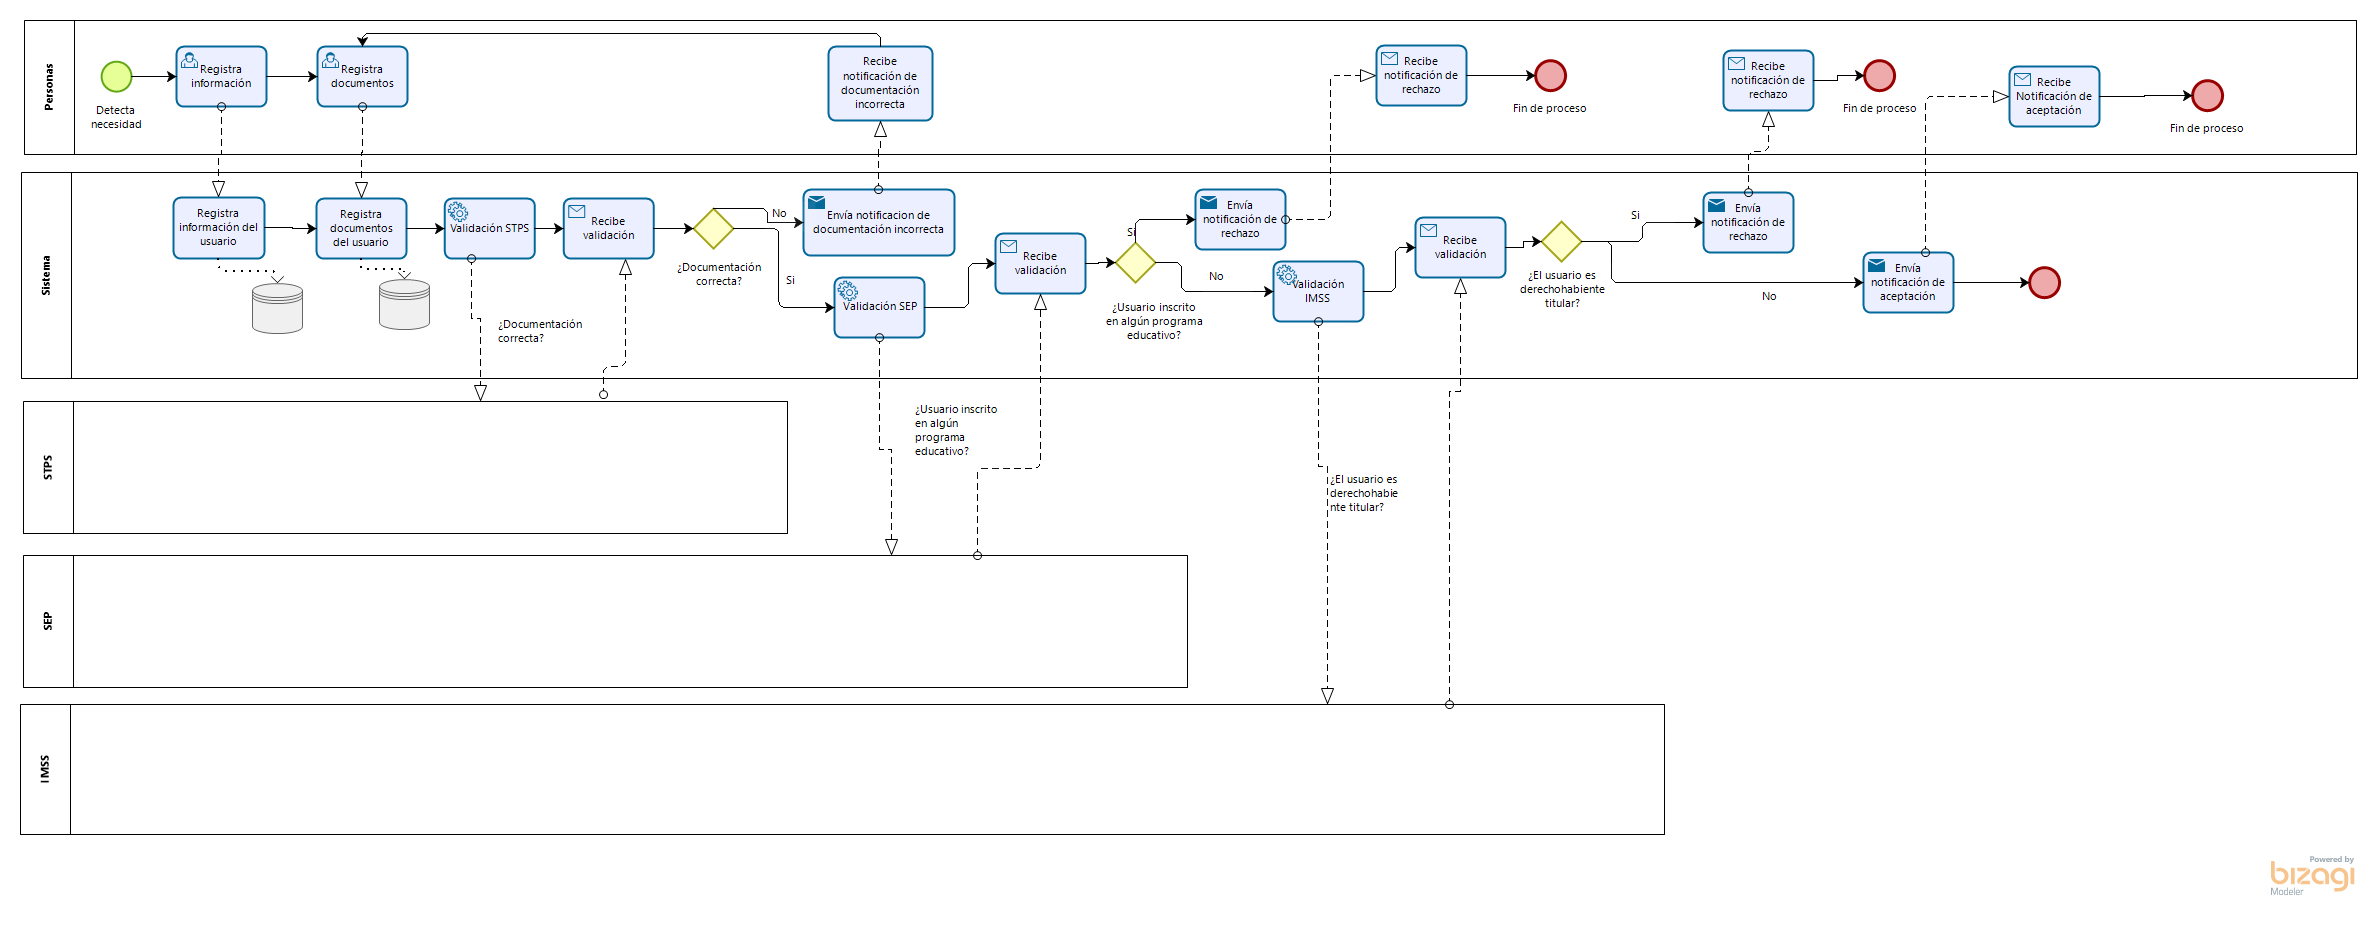
\includegraphics[angle=90,  width=0.4\textwidth]{marcoTeorico/imagenes/Proceso_RegistroPersonas.png}
\caption{Proceso ``Registro de persona''}
\end{center}
\end{figure}

\textbf{Descripción} \\

El proceso comienza cuando un becario (en este caso un NINI) detecta la necesidad de incorporarse al campo laboral, el usuario becario realiza una solicitud de registro al sistema, ingresa su información y anexa los documentos que validan su identidad y la información registrada. Ya que el sistema almacena la información, una vez que los documentos se encuentran registrados se comienza la validación con los servicios web simulados, los cuales se encargan de validar la información.\\
\\Los servicios web simulados son el de la SEP( Secretaria de Educación Pública), el del IMSS (Instituto Mexicano del Seguro Social) y la STPS (Secretaría del Trabajo y Prevención Social), una vez que se valida la información por medio de los servicios web, el sistema procede a asignarle el estado de aceptación o de rechazo al usuario. %se validan los documentos con la secretaria del Trabajo y Prevención Social (STPS) la cual valida los documentos, si los documentos son válidos 
%se procede a realizar peticiones a servicios web  que simularán la validación de la información del usuario con la SEP y el IMSS, dependiendo de la respuestas de los servicios se asigna el estado de aceptación o rechazo al usuario, una vez que el usuario es aceptado se registra en el sistema el estatus del NINI. %finalmente se ejecuta el subproceso de perfilamiento y se registra el perfil del NINI \\
\\


%\textbf{Tabla de Elementos del proceso}

%\begin{table}[htb]
%\centering
%\begin{tabular}{|l|l|}
%\hline
%\multicolumn{2}{|c|}{\textbf{Proceso Registro de Persona}} \\ \hline
%\textbf{Procesos que dependen del proceso} &  Asignación \\ \hline

%\textbf{Dependencia de otros procesos} & Proceso de perfilamiento  \\  \hline

%\multirow{2}{3cm}{\textbf{Entradas}} & Datos del NINI \\ \cline{2-2}
%& Documentos para validar información \\ \hline

%\textbf{Salidas} & Notificaciones \\ \hline

%\textbf{Precondiciones} &  \\ \hline

%\textbf{Postcondiciones} & Persona registrada \\ \hline

%\end{tabular}
%\caption{Tabla de elementos Registro de persona.}
%\label{tabla:sencillaPersonas}
%\end{table}


